% !TeX program = xelatex
% Recommended build:
%   latexmk -xelatex -bibtex -interaction=nonstopmode main.tex
\documentclass[11pt,a4paper]{article}

\usepackage{fontspec}
\usepackage{ucharclasses}
\usepackage{amsmath,amssymb,mathtools,bm}
\usepackage{geometry}
\usepackage{setspace}
\usepackage{xcolor}
\usepackage{booktabs,longtable,tabularx,array,multirow,makecell}
\usepackage{enumitem}
\usepackage{titlesec}
\usepackage{fancyhdr,lastpage}
\usepackage{caption}
\usepackage{float}
\usepackage{graphicx}
\usepackage{adjustbox}
\usepackage{tcolorbox}
\tcbuselibrary{breakable,skins}
\usepackage[numbers,sort&compress]{natbib}
\usepackage{xurl}
\usepackage{hyperref}

% ---------- Fonts ----------
% Chinese body: Song-style; Chinese headings: Hei-style.
% Latin: bundled Nimbus Roman/Sans, Times/Helvetica-compatible metrics.
\defaultfontfeatures{Ligatures=TeX}
\setmainfont{NotoSerifSC-Regular.ttf}[
  Path=fonts/,
  BoldFont=NotoSerifSC-Bold.ttf,
  ItalicFont=NotoSerifSC-Regular.ttf,
  BoldItalicFont=NotoSerifSC-Bold.ttf,
  ItalicFeatures={FakeSlant=0.16},
  BoldItalicFeatures={FakeSlant=0.16}
]
\setsansfont{NotoSansSC-Regular.ttf}[
  Path=fonts/,
  BoldFont=NotoSansSC-Bold.ttf
]
\setmonofont{Latin Modern Mono}
\newfontfamily\latinserif{NimbusRoman-Regular.otf}[
  Path=fonts/,
  BoldFont=NimbusRoman-Bold.otf,
  ItalicFont=NimbusRoman-Italic.otf,
  BoldItalicFont=NimbusRoman-BoldItalic.otf
]
\newfontfamily\latinsans{NimbusSans-Regular.otf}[
  Path=fonts/,
  BoldFont=NimbusSans-Bold.otf,
  ItalicFont=NimbusSans-Italic.otf,
  BoldItalicFont=NimbusSans-BoldItalic.otf
]
\newfontfamily\cnserif{NotoSerifSC-Regular.ttf}[
  Path=fonts/,
  BoldFont=NotoSerifSC-Bold.ttf,
  ItalicFont=NotoSerifSC-Regular.ttf,
  BoldItalicFont=NotoSerifSC-Bold.ttf,
  ItalicFeatures={FakeSlant=0.16},
  BoldItalicFeatures={FakeSlant=0.16}
]
\newfontfamily\cnsans{NotoSansSC-Regular.ttf}[
  Path=fonts/,
  BoldFont=NotoSansSC-Bold.ttf
]
\setTransitionsForLatin{\latinserif}{\cnserif}
\newcommand{\headingfonts}{%
  \cnsans
  \setTransitionsForLatin{\latinsans}{\cnsans}%
  \cnsans
}
\XeTeXlinebreaklocale "zh"
\XeTeXlinebreakskip=0pt plus 1pt

% ---------- Page and journal styling ----------
\geometry{left=2.2cm,right=2.2cm,top=2.2cm,bottom=2.2cm,headheight=15pt}
\setstretch{1.625}
\setlength{\parindent}{2em}
\setlength{\parskip}{0pt}
\setlength{\emergencystretch}{2em}
\renewcommand{\arraystretch}{1.18}
\setlist{nosep,leftmargin=2em}
\setlist[itemize]{label=$\bullet$}

\definecolor{DeepBlue}{HTML}{17365D}
\definecolor{MainBlue}{HTML}{1D4E89}
\definecolor{SoftBlue}{HTML}{EEF5FC}
\definecolor{SoftGray}{HTML}{F4F5F7}
\definecolor{RuleGray}{HTML}{BFC7D1}
\definecolor{GainGreen}{HTML}{2F7D4A}
\definecolor{WarnRed}{HTML}{A33A3A}

\titleformat{\section}
  {\headingfonts\Large\bfseries\color{DeepBlue}}
  {\thesection}{0.7em}{}
\titleformat{\subsection}
  {\headingfonts\large\bfseries\color{MainBlue}}
  {\thesubsection}{0.7em}{}
\titleformat{\subsubsection}
  {\headingfonts\normalsize\bfseries}
  {\thesubsubsection}{0.6em}{}
\titlespacing*{\section}{0pt}{1.45em}{0.55em}
\titlespacing*{\subsection}{0pt}{1.15em}{0.40em}
\titlespacing*{\subsubsection}{0pt}{0.90em}{0.30em}

\pagestyle{fancy}
\fancyhf{}
\fancyhead[L]{\small 安全多布局组合量子比特路由}
\fancyhead[R]{\small Safe Multi-Layout Portfolio Routing}
\fancyfoot[C]{\small \thepage/\pageref{LastPage}}
\renewcommand{\headrulewidth}{0.4pt}
\renewcommand{\footrulewidth}{0pt}

\renewcommand{\abstractname}{摘\quad 要}
\renewcommand{\refname}{参考文献}
\renewcommand{\figurename}{图}
\renewcommand{\tablename}{表}
\captionsetup{
  font={small,bf},
  labelfont=bf,
  labelsep=quad,
  justification=centering,
  singlelinecheck=false
}

\hypersetup{
  colorlinks=true,
  linkcolor=DeepBlue,
  citecolor=MainBlue,
  urlcolor=MainBlue,
  pdftitle={安全多布局组合量子比特路由：完整策略展开、跨布局迁移与可审计选择},
  pdfauthor={Anonymous Author},
  pdfsubject={Qubit routing, LightSABRE, multi-layout portfolio, safe selection},
  pdfkeywords={量子比特路由, LightSABRE, 多布局组合, 安全选择, 盲测}
}

% ---------- Math and reusable environments ----------
\newcommand{\Hardware}{\mathcal H}
\newcommand{\Circuit}{\mathcal C}
\newcommand{\Front}{\mathcal F}
\newcommand{\Extended}{\mathcal X}
\newcommand{\Candidates}{\mathcal A}
\newcommand{\Portfolio}{\mathcal P}
\newcommand{\RouteDist}{\delta_{\Hardware}}
\newcommand{\DepthW}{D_{\mathrm w}}
\newcommand{\argmin}{\operatorname*{arg\,min}}
\newcommand{\Drain}{\operatorname{Drain}}
\newcommand{\LS}{\mathrm{LS}}
\newcommand{\Rollout}{\mathrm{Rollout}}
\newcommand{\SMPR}{\mathrm{SMPR}}
\newcommand{\CrossLayout}{\mathrm{CrossLayout}}
\newcommand{\BaselineRollout}{\mathrm{BaselineRollout}}

\newtcolorbox{claimbox}[1][]{
  breakable,
  enhanced,
  colback=SoftBlue,
  colframe=MainBlue,
  boxrule=0.7pt,
  arc=1.2mm,
  left=2mm,right=2mm,top=1.5mm,bottom=1.5mm,
  #1
}
\newtcolorbox{notebox}[1][]{
  breakable,
  enhanced,
  colback=SoftGray,
  colframe=RuleGray,
  boxrule=0.6pt,
  arc=1.2mm,
  left=2mm,right=2mm,top=1.5mm,bottom=1.5mm,
  #1
}
\newtcolorbox{algobox}[1]{
  breakable,
  enhanced,
  title={#1},
  fonttitle=\bfseries,
  coltitle=white,
  colback=white,
  colframe=DeepBlue,
  colbacktitle=DeepBlue,
  boxrule=0.7pt,
  arc=1.2mm,
  left=2.5mm,right=2.5mm,top=1.5mm,bottom=1.5mm
}

\newcolumntype{Y}{>{\raggedright\arraybackslash}X}
\newcolumntype{C}[1]{>{\centering\arraybackslash}p{#1}}
\newcolumntype{R}[1]{>{\raggedleft\arraybackslash}p{#1}}

\begin{document}

\begin{center}
  {\headingfonts\fontsize{20}{28}\selectfont\bfseries
  安全多布局组合量子比特路由：完整策略展开、跨布局迁移与可审计选择\par}
  \vspace{0.55em}
  {\latinsans\large\bfseries
  Safe Multi-Layout Portfolio Routing for Connectivity-Constrained\\
  Quantum Circuits\par}
  \vspace{1.0em}
  {\large Anonymous Author\textsuperscript{1}\par}
  \vspace{0.25em}
  {\small \textsuperscript{1}Author affiliation omitted for double-blind review\par}
  \vspace{0.25em}
  {\small 通信信息将在双盲结束后补充\par}
  \vspace{0.25em}
  {\small SMPR public-core 1.0.0-rc3 / V5--V7 verified evidence\par}
\end{center}

\vspace{0.4em}
\begin{abstract}
\begin{spacing}{1.38}
受限耦合拓扑要求量子编译器通过动态逻辑--物理映射插入 SWAP，但强基线的随机布局、多步路由决策与工程开销之间存在明显张力。本文提出安全多布局组合路由器（Safe Multi-Layout Portfolio Router，SMPR）：以 20 个随机种子的 LightSABRE 为显式质量下界，使用完整基线策略展开生成互补路由候选，并将 LightSABRE 并列最优初始布局及其代理筛选的一换位邻域重新路由；最终按 $(\text{SWAP},\text{加权深度})$ 字典序选择，完全同质时优先 LightSABRE。由于候选集中始终包含 LightSABRE，SMPR 在指标实现一致的前提下具有结构性的逐实例不退化保证。为避免候选组合被解释器和 Qiskit 重复导入开销淹没，本文进一步设计四个长生命周期分片进程和最长处理时间优先调度。

算法冻结后，我们在 120 个预注册 V6 盲测实例上进行主要推断。SMPR 将总 SWAP 从 3176 降至 3051，减少 125 个（3.94\%）；逐实例胜/平/负为 50/70/0。以每例 CX 数归一化的配对差值均值为 $-0.018727$，10\,000 次实例级 bootstrap 的 95\% 置信区间为 $[-0.024346,-0.013634]$，上端低于零；按 60 个因子单元分组重采样的补充稳健区间为 $[-0.024392,-0.013594]$。语义、拓扑和指标审计均为 120/120。2026-07-25 的独立环境复现再次得到 V5/V6 总量和联合统计审计。随后执行的 V7 前瞻性外部验证使用 10 条 QASMBench 公共线路、11--23 个逻辑比特和 19/57 比特 heavy-hex，在三次同机重复中形成 120 条配对观测。相对时间匹配 LightSABRE，SMPR 在 $0.25T,0.5T,T,2T$ 四档预算下分别减少 11.05\%、8.84\%、7.30\% 和 5.17\% 的总 SWAP；四个按线路聚类的 95\% 区间均轻微跨越零，故该结果是外部汇总优势证据，而非 95\% 水平下的显著性结论。V7 的冻结清单、三个重复哈希、环境记录以及 120/120 路由轨迹、拓扑和安全下界审计全部通过。独立的自适应展开分支在 V6 上弱于 LightSABRE；因此，证据支持安全组合与跨布局迁移，而非某个单一路由器的普遍支配。
\end{spacing}

\noindent\textbf{关键词：}量子比特路由；量子编译；LightSABRE；策略展开；初始布局；算法组合；盲测
\end{abstract}

\begin{notebox}[title={English abstract}]
\begin{spacing}{1.08}
\footnotesize
\textbf{Abstract.}
We present the Safe Multi-Layout Portfolio Router (SMPR) for
connectivity-constrained quantum compilation.  Twenty-seed LightSABRE is
retained as an explicit quality floor.  An adaptive-rollout branch uses full
baseline-policy rollout, while a cross-layout branch reroutes every
unique LightSABRE initial layout tied at the best $(\mathrm{SWAP},D_{\mathrm w})$
quality, together with four proxy-ranked one-transposition neighbors.  The
final candidate is selected lexicographically by $(\mathrm{SWAP},D_{\mathrm w})$,
with LightSABRE preferred on an exact tie.  On the preregistered 120-instance
V6 blind set, the portfolio reduces total SWAPs from 3176 to 3051 (3.94\%),
with a per-instance win/tie/loss record of 50/70/0.  The mean paired gap
normalized by the number of CX gates is $-0.018727$; its 10\,000-sample
bootstrap 95\% confidence interval is $[-0.024346,-0.013634]$.  All semantic,
topological, and metric audits pass.  The standalone adaptive-rollout branch
is weaker than LightSABRE, so the evidence supports safe portfolio compilation and
cross-layout transfer rather than universal dominance by a standalone router.
An independent clean-directory reproduction revalidated all V5/V6 totals,
the joint statistical audit, and all 18 archived evidence hashes.  A
prospectively frozen V7 evaluation further covers ten public QASMBench
circuits, 11--23 logical qubits, and 19/57-qubit heavy-hex graphs.  Across
three same-machine repeats, SMPR uses 11.05\%, 8.84\%, 7.30\%, and 5.17\%
fewer aggregate SWAPs than time-matched LightSABRE at budgets
$0.25T,0.5T,T,$ and $2T$, respectively.  The four circuit-clustered 95\%
intervals slightly cross zero, so V7 supports an aggregate external trend,
not a 95\%-level significance claim.  All 120 routing-trace, topology, and
internal-quality-floor audits pass.

\noindent\textbf{Keywords:} qubit routing; quantum compilation; LightSABRE;
policy rollout; initial layout; safe portfolio; blind evaluation
\end{spacing}
\end{notebox}

\section{引言}

当前量子程序通常在逻辑量子比特之间自由描述双比特门，而真实设备只允许耦合图上相邻的物理量子比特直接交互。编译器因而必须联合决定初始布局与运行时映射更新，并以 SWAP 将不可执行的逻辑门转化为硬件合法操作。该问题与寄存器分配、token swapping 和受约束调度相关，通常具有难以承受的精确求解代价，因此实践系统依赖启发式搜索\citep{Siraichi2018QubitAllocation,Zulehner2018Mapping,Cowtan2019Routing}。

SABRE 通过双向布局、动态前沿和距离启发式在质量与复杂度之间取得了有影响力的平衡\citep{Li2019SABRE}。LightSABRE 进一步利用相对评分、多试验、关键路径项和高效实现显著提升可扩展性\citep{Zou2024LightSABRE}。这使研究型路由器面临两个现实问题。第一，单一启发式即使在部分实例上更强，也可能在其他实例上明显退化；只报告平均值容易掩盖风险。第二，更深的候选展开、多个初始布局和语义验证会放大 Python 进程启动与依赖导入开销，使算法质量与执行工程相互纠缠。

本文报告 SMPR 从候选生成、质量选择到导出审计的完整、冻结且经盲测验证的技术路径。核心观察是：强随机化基线与完整策略展开的优势并非严格替代关系。独立自适应展开分支在冻结 V6 上比 LightSABRE 多 210 个 SWAP，但若从 LightSABRE 找到的优质布局出发，尤其在该布局的一换位邻域中重新路由，则能产生新的优胜解。因此，本文将布局发现与路由策略视为可重新组合的两个模块，并始终保留强基线作为质量下界。

本文主要贡献如下。

\begin{enumerate}[label=(\arabic*),itemsep=0.35em]
  \item 提出一种\textbf{完整基线策略展开}的路由决策。候选 SWAP 先经历“交换--闭包执行”，再由冻结基线策略完成余下线路；仅当最优候选的剩余 SWAP 严格少于基线候选时改变动作，从而抑制短视启发式造成的局部后悔。
  \item 提出一种\textbf{跨布局迁移}机制。它收集 20 次 LightSABRE 中在 $(\mathrm{SWAP},\DepthW)$ 上并列最优的全部唯一初始布局，对每个布局及其 4 个代理最优的一换位邻居运行真实完整路由，而不是以代理分数直接决定输出。
  \item 构造\textbf{安全组合选择规则}。LightSABRE 始终在候选集中，最终按以 SWAP 和加权深度为首两项的冻结五元键选择；因而输出在逐实例 SWAP 上不可能劣于 LightSABRE，等 SWAP 时深度也不劣。
  \item 建立\textbf{导出后审计链}。所有最终 QASM 均检查逻辑--物理映射、Clifford 语义等价、耦合边合法性、加权深度和 SWAP/CX 计数，并记录 SHA-256。
  \item 通过\textbf{预注册 V6 盲测}给出主要统计结论，并将 V5 限定为工程复核；进一步以前瞻冻结的 V7 公共线路和 heavy-hex 实验给出同机质量--时间外部验证，同时保持确认性结论与探索性外部证据的层级区分。
\end{enumerate}

\begin{claimbox}[title={本文的证据边界}]
本文支持的确认性主张是：“冻结的 SMPR 在 V6 盲测上显著减少 SWAP，且逐实例无 SWAP 退化。”V7 进一步支持“在四档同机匹配预算下观察到总 SWAP 优势”，但其按公共线路聚类的 95\% 区间跨零，不能写成统计显著的普遍优势。本文不支持“独立自适应展开分支普遍优于 LightSABRE”，也不支持“SMPR 在所有线路上更快或更优”。
\end{claimbox}

\section{问题定义与评价指标}

\subsection{受限拓扑上的路由}

设逻辑线路为有向无环依赖图
\begin{equation}
  \Circuit=(Q,G,E_{\Circuit}),
\end{equation}
其中 $Q$ 为逻辑量子比特集合，$G$ 为门集合，$E_{\Circuit}$ 表示数据依赖。硬件由无向耦合图
\begin{equation}
  \Hardware=(V,E_{\Hardware}),\qquad |V|\ge |Q|
\end{equation}
表示。时刻 $t$ 的逻辑到物理单射记为 $\pi_t:Q\rightarrow V$。双比特门 $g(q_i,q_j)$ 可执行，当且仅当
\begin{equation}
  \{\pi_t(q_i),\pi_t(q_j)\}\in E_{\Hardware}.
  \label{eq:executable}
\end{equation}
在硬件边 $(u,v)\in E_{\Hardware}$ 上插入 SWAP 会交换占据 $u,v$ 的逻辑量子比特并更新 $\pi_t$。路由器的首要目标是减少新增 SWAP 数
\begin{equation}
  S(C')=N_{\mathrm{SWAP}}(C'),
\end{equation}
其中 $C'$ 是物理线路。

\subsection{加权深度与字典序质量}

本文用资源占用式调度定义加权深度。每条物理线维护完成时刻 $d_v$。对作用于集合 $U_g$ 的门 $g$，令
\begin{equation}
  f(g)=\max_{v\in U_g}d_v+w(g),\qquad
  w(g)=
  \begin{cases}
    3,&g=\mathrm{SWAP},\\
    1,&\text{其他一、双比特门},
  \end{cases}
  \label{eq:weighted-depth}
\end{equation}
并将 $U_g$ 上的完成时刻更新为 $f(g)$。最终
\begin{equation}
  \DepthW(C')=\max_{v\in V}d_v.
\end{equation}
SWAP 权重 3 与其分解为 3 个 CX 的导出口径一致。候选质量定义为
\begin{equation}
  \mathbf q(c)=\bigl(S(c),\DepthW(c)\bigr),
  \label{eq:quality}
\end{equation}
并采用字典序最小化：SWAP 为主目标，深度只在 SWAP 相同时破平。

\subsection{配对统计量}

对实例 $i$，设组合路由器和 LightSABRE 的 SWAP 分别为 $S_i^{P}$ 与 $S_i^{L}$，输入 CX 数为 $M_i$。预注册主统计量为
\begin{equation}
  \bar{\Delta}
  =\frac{1}{N}\sum_{i=1}^{N}
  \frac{S_i^{P}-S_i^{L}}{M_i}.
  \label{eq:normalized-gap}
\end{equation}
负值表示组合路由器更优。V6 在算法冻结前约定：对 $N=120$ 个配对差值进行 10\,000 次有放回重采样，随机种子固定为 20260723；若 95\% percentile bootstrap 区间上端小于 0，则主要推断通过\citep{Efron1979Bootstrap}。

\section{相关工作}

早期工作将逻辑量子比特映射到受限架构视为编译期分配与路由问题。Siraichi 等讨论了 qubit allocation 的程序表示与求解策略\citep{Siraichi2018QubitAllocation}；Zulehner 等针对 IBM QX 架构提出基于搜索的映射方法\citep{Zulehner2018Mapping}；Cowtan 等从架构无关角度研究了路由方法和双比特门开销\citep{Cowtan2019Routing}。这些工作共同说明，布局和动态移动不能只作为彼此独立的后处理步骤。

SABRE 使用前沿层与扩展集上的物理距离评分候选 SWAP，并以反向遍历改善初始布局\citep{Li2019SABRE}。LightSABRE 在 Qiskit 中加入相对评分、多试验、可扩展实现及停滞释放机制，是本文最重要的工程基线\citep{Zou2024LightSABRE,JavadiAbhari2024Qiskit}。LightSABRE 的多试验结果也揭示了布局随机性：同一路由策略因初始布局不同可能产生明显质量差异。

另一条路线通过局部搜索、束搜索、蒙特卡洛树搜索或强化学习提升搜索深度\citep{Luo2025LocalSearch,Zhou2020MCTS,Herbert2022RLRouter}。这类方法的共同难点是代理函数与完整线路质量之间存在偏差。本文的完整策略展开与 rollout policy improvement 类似：以一个确定基线策略评估候选动作的余下 SWAP，而不是无限增加启发式项。与只运行多个完整路由器后取最优不同，本文还把 LightSABRE 发现的布局作为可迁移中间表示，并在其局部邻域中调用另一策略。

组合方法在经典算法工程中常用于吸收不同求解器的互补性。本文的特殊之处是显式保留强基线候选，由此获得可证明的指标下界；同时，每个输出都通过可执行线路级审计，而非只比较内部计数。QASM 3 与 Qiskit 提供了导出和重载基础\citep{Cross2022OpenQASM3,JavadiAbhari2024Qiskit}，Clifford 表示则使本文使用的 $\{H,\mathrm{CX},\mathrm{SWAP}\}$ 基准线路能够进行精确等价比较\citep{Aaronson2004Clifford}。

\section{方法}

\subsection{总体架构}

图~\ref{fig:architecture} 展示 SMPR 的数据流。LightSABRE 分支既产生强基线，也提供可迁移布局；独立展开分支保留自身布局策略；跨布局分支在 LightSABRE 的并列最优布局及其邻域上运行同一完整展开策略。三个分支均产生真实路由结果，最终统一按同一质量口径选择和审计。

\begin{figure}[H]
\centering
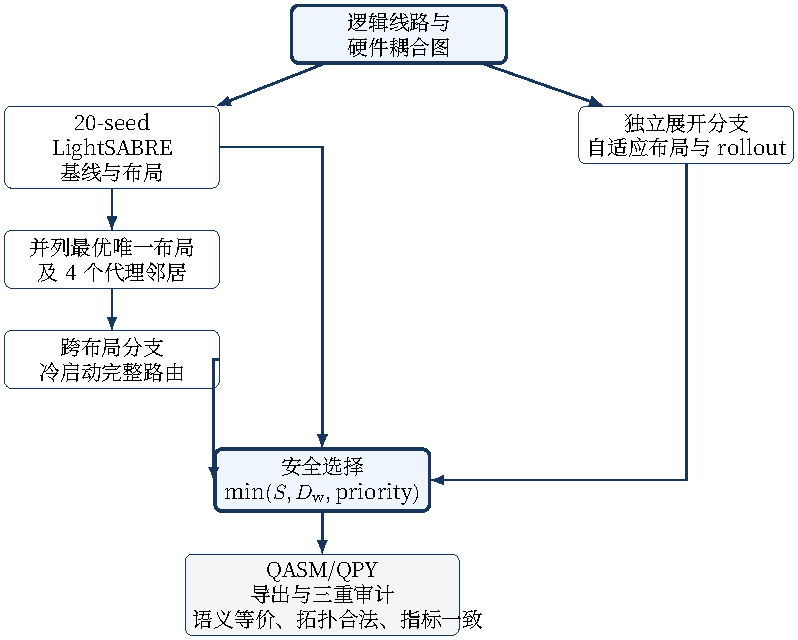
\includegraphics[width=0.82\textwidth]{figures/fig_architecture.pdf}
\caption{安全多布局组合路由器 SMPR 的总体架构}
\label{fig:architecture}
\end{figure}

\begin{algobox}{算法 1：SMPR 总流程}
\begin{enumerate}[label=\arabic*.,leftmargin=2.3em,itemsep=0.18em]
  \item \textbf{输入：}逻辑线路 $\Circuit$、耦合图 $\Hardware$、LightSABRE 种子数 $r$、展开宽度 $k$、每布局邻居数 $b$ 与布局代理衰减 $\gamma$。
  \item 运行 $r$ 个 LightSABRE 试验，保存每个候选的初始布局、物理线路、SWAP、加权深度与审计信息；将最佳候选加入 $\Portfolio$。
  \item 使用自身冻结布局池运行独立自适应展开分支，将其最佳真实路由结果加入 $\Portfolio$。
  \item 收集 LightSABRE 中质量并列最优的唯一布局；对每个布局枚举一换位邻域，按 $P_\gamma$ 保留前 $b$ 个。
  \item 从每个基布局及保留邻居冷启动完整路由；所有去重后的真实路由结果均加入 $\Portfolio$。
  \item 按式~\eqref{eq:deterministic-key} 选择 $c^*$，导出线路并执行语义、拓扑与指标审计；任一审计未通过则不输出该线路。
  \item \textbf{输出：}物理线路、初始/最终映射、质量二元组、候选来源、审计记录与内容哈希。
\end{enumerate}
\end{algobox}

\subsection{自适应展开分支的状态、势函数与候选集}

路由状态包含当前映射 $\pi$、逆映射、DAG 剩余入度、已执行门集合、动态前沿、物理线完成时刻以及最近一次 SWAP。每次决策前，$\Drain$ 反复执行所有依赖满足且符合式~\eqref{eq:executable} 的门，直到没有新门可执行。这一闭包使候选动作的收益反映其连续解锁能力，而不是只看交换后的瞬时距离。

对双比特门 $g(q_i,q_j)$，定义路由距离
\begin{equation}
  \RouteDist(g,\pi)
  =d_{\Hardware}\bigl(\pi(q_i),\pi(q_j)\bigr)-1,
\end{equation}
其中 $d_{\Hardware}$ 为耦合图最短路长度。相邻门的路由距离为 0。冻结的有序长前瞻势函数为
\begin{equation}
  \Phi(s)
  =\sum_{g\in \Front(s)}\RouteDist(g,\pi_s)
  +\sum_{i=0}^{|\Extended(s)|-1}2^{-i}
   \RouteDist\bigl(\Extended_i(s),\pi_s\bigr).
  \label{eq:potential}
\end{equation}
$\Extended(s)$ 通过以当前前沿为根的 DAG 广度优先遍历生成，只记录随后暴露的双比特门。其动态上限为
\begin{equation}
  h(s)=\min\left\{b(\bar d)+
  \left\lfloor\frac{R_2(s)}{20}\right\rfloor,1000\right\},
\end{equation}
其中 $R_2(s)$ 为剩余双比特门数，硬件平均度 $\bar d\ge3.5$、$2.5\le\bar d<3.5$、$\bar d<2.5$ 时，$b(\bar d)$ 分别为 250、300、400。稀疏拓扑获得更长观察窗口。

候选集合 $\Candidates(s)$ 包含两类硬件边：（1）与 $\Front(s)\cup\Extended(s)$ 中任一门的物理端点相接的边；（2）对每个相关门，在一条确定最短路径上的全部边。该集合比只围绕当前前沿端点生成候选更宽，同时避免枚举无关硬件边。

对候选 SWAP $a$，深复制状态，应用 $a$ 并执行 $\Drain$。设 $\Delta\Phi_a=\Phi(s_a)-\Phi(s)$，新执行双比特门集合为 $U_a$。根据 DAG 关键性权重 $\omega_g$ 计算
\begin{equation}
  H(s,a)=\Delta\Phi_a
  -\beta\sum_{g\in U_a}\omega_g
  +\rho\,\mathbb I(a=a_{\mathrm{last}}),
  \label{eq:heuristic}
\end{equation}
冻结参数为 $\beta=2.0$、$\rho=0$，关键性衰减参数为 $\alpha=0.5$。候选排序键依次为
\begin{equation}
  \bigl(H,\,-\text{unlock},\,\Delta\Phi,\,
  \Delta\DepthW,\,\text{edge}\bigr).
  \label{eq:candidate-key}
\end{equation}

\subsection{完整基线策略展开}

单步启发式可能偏好立即降低距离、却使后续线路支付更多 SWAP。为估计这一后果，本文对启发式排序后的前 $k$ 个候选进行完整基线策略展开。记冻结基线策略为 $\pi_0$，候选 $a$ 后经闭包得到状态 $T(s,a)$，则
\begin{equation}
  Q^{\pi_0}(s,a)
  =1+V^{\pi_0}\bigl(T(s,a)\bigr),
  \label{eq:rollout-q}
\end{equation}
其中 $V^{\pi_0}$ 是从后继状态按 $\pi_0$ 完成线路所需的剩余 SWAP 数。状态指纹与最近动作共同用于缓存完整展开结果。

设 $a_0=\pi_0(s)$ 为基线动作，$\hat a$ 是候选集合中 $Q^{\pi_0}$ 最小的动作。实际决策为
\begin{equation}
  a^*(s)=
  \begin{cases}
    \hat a,&Q^{\pi_0}(s,\hat a)<Q^{\pi_0}(s,a_0),\\
    a_0,&\text{其他}.
  \end{cases}
  \label{eq:strict-improvement}
\end{equation}
相同剩余 SWAP 时保持基线动作，避免等价 $Q$ 值在逐步重规划中形成无意义循环；深度仅稳定 rollout 内部排序。通常 $k=2$，仅对冻结的 grid、$n=10$、alternating 变体取 $k=4$。

\begin{algobox}{算法 2：完整基线策略展开的一步决策}
\begin{enumerate}[label=\arabic*.,leftmargin=2.3em,itemsep=0.18em]
  \item 在状态 $s$ 上构造 $\Front,\Extended,\Candidates$，按式~\eqref{eq:candidate-key} 排序；记首项为基线动作 $a_0$。
  \item 保留前 $k$ 项，并确保 $a_0$ 在集合中。
  \item 对每个 $a$：应用 SWAP，执行 $\Drain$，再用冻结策略 $\pi_0$ 完成线路；缓存并返回 $Q^{\pi_0}(s,a)$。
  \item 取 $Q^{\pi_0}$ 最小的 $\hat a$。若其 SWAP 严格少于 $a_0$，执行 $\hat a$；否则执行 $a_0$。
  \item 从新状态重新生成候选，直到全部逻辑门执行完毕。
\end{enumerate}
\end{algobox}

\subsection{独立展开分支的自适应布局}

独立展开分支不是单一初始布局。默认实例使用冻结的自适应映射策略：parallel\_layers 线路采用完整映射池，其余线路采用 v1\_best 映射，均以 $k=2$ 展开。三个结构化困难子类使用冻结专门规则：

\begin{table}[H]
\centering
\small
\caption{独立展开分支的冻结布局变体}
\label{tab:native-variants}
\begin{tabularx}{\textwidth}{p{0.30\textwidth}p{0.24\textwidth}Y}
\toprule
触发条件 & 路由展开 & 布局策略 \\
\midrule
ring，$n=10$，far & $k=2$ &
束宽 2、1 轮局部搜索，保留 2 个布局做完整路由。\\
grid，$n\ge8$，uniform & $k=2$ &
衰减 0.95 的布局代理，代理前 8 中选 2 个做完整路由。\\
grid，$n=10$，alternating & $k=4$ &
同上，但路由候选展开宽度增至 4。\\
其他 & $k=2$ &
默认自适应映射预算。\\
\bottomrule
\end{tabularx}
\end{table}

为保持冻结基线逐例一致，独立展开分支在同一硬件对象上先运行一次基线策略，再执行 rollout；该过程也预热最短路缓存。跨布局分支被视为独立候选来源，采用冷启动，二者不可在审计时混为一谈。

\subsection{交叉布局与一换位邻域}

LightSABRE 使用随机性搜索布局和路由。对每个实例运行种子 $0,\ldots,19$，每个种子重复 1 次。设 20 个候选中的最优质量为 $\mathbf q_L^*$，收集所有满足
\begin{equation}
  \mathbf q(c)=\mathbf q_L^*
\end{equation}
的候选。冻结证据实现按运行时间和种子排序后以初始映射去重；正式算法规则则按种子、映射和标签确定性排序。冻结参数 \texttt{cross-layout-bases=0} 表示保留全部并列最优唯一布局，而不是零个布局。

对每个布局 $\pi$，按输入 CX 的顺序定义代理
\begin{equation}
  P_{\gamma}(\pi)
  =\sum_{i=0}^{M-1}\gamma^i
  d_{\Hardware}\bigl(\pi(q_i),\pi(q'_i)\bigr),
  \qquad \gamma=0.95.
  \label{eq:layout-proxy}
\end{equation}
枚举交换任意两个逻辑量子比特物理位置的一换位邻域
\begin{equation}
  \mathcal N_1(\pi)
  =\{\pi\circ(i\,j)\mid 0\le i<j<n\},
\end{equation}
按 $(P_{\gamma},\text{mapping})$ 排序并保留前 4 个。最终对基布局及这 4 个邻居逐一运行真实完整路由，映射重复时去重。代理只用于分配昂贵完整路由预算，不直接参与最终质量选择。

该机制与“修改 LightSABRE 已输出的物理线路”不同：传递的是\textbf{初始布局}，每个跨布局候选都从原始逻辑线路重新完整路由。因此，最终收益来自“一个分支发现布局、另一个分支解释布局”的跨策略组合。

\subsection{安全组合选择}

每个实例的候选集合为
\begin{equation}
  \Portfolio
  =\Portfolio_{\LS}
  \cup\Portfolio_{\Rollout}
  \cup\Portfolio_{\CrossLayout}.
\end{equation}
正式算法规则的确定性排序键为
\begin{equation}
  K_{\mathrm d}(c)=
  \bigl(S(c),\DepthW(c),p(c),\sigma(c),m(c),\ell(c)\bigr),
  \label{eq:deterministic-key}
\end{equation}
其中 $p(\LS)=0$、$p(\CrossLayout)=1$、$p(\Rollout)=2$，$\sigma$ 为随机种子（无种子时取固定最大 sentinel 值），$m$ 为初始映射的标准元组，$\ell$ 为候选标签。完全相同的 SWAP 和深度下优先 LightSABRE，因为其原生 QPY 更直接且候选生成成本通常更低。后四项仅用于确定性破平，不改变前两项的质量定义。

\paragraph{命题 1（安全质量下界）}
若 $\Portfolio$ 包含 LightSABRE 最优候选 $c_L$，并按式~\eqref{eq:deterministic-key} 选择 $c^*$，则
\begin{equation}
  S(c^*)\le S(c_L).
\end{equation}
若 $S(c^*)=S(c_L)$，则 $\DepthW(c^*)\le\DepthW(c_L)$。

\paragraph{证明}
由 $c^*=\argmin_{c\in\Portfolio}K(c)$ 且 $c_L\in\Portfolio$，有
$K(c^*)\le_{\mathrm{lex}}K(c_L)$。比较前两维即得结论。\hfill$\square$

命题 1 是选择结构的性质，不依赖任何互补分支单独是否强于基线。它解释了盲测中的 0 个逐实例 SWAP 退化；审计链则保证“内部质量键”与真实导出线路一致。

\paragraph{冻结证据实现与正式规则的边界}
V5/V6 冻结程序使用既有键
\begin{equation}
  K_{\mathrm f}(c)=
  \bigl(S(c),\DepthW(c),p(c),t(c),\ell(c)\bigr),
  \label{eq:frozen-key}
\end{equation}
其中 $t$ 为实测运行时间。式~\eqref{eq:frozen-key} 与
式~\eqref{eq:deterministic-key} 的前三项完全相同，因此既有总 SWAP、加权深度、
后端类别和命题 1 均按冻结证据原样报告；但两式可能在同质量、同来源候选内部
选择不同的具体线路。公开核心把两种模式显式分开：冻结兼容配置用于复现
V5/V6，确定性配置用于新的算法版本。后者在替代冻结配置前必须接受新的盲测，
不能用 V6 重新调参后再把 V6 称为未见数据。

\subsection{计算复杂度与预算}

设物理量子比特数为 $n$，输入双比特门数为 $M$，LightSABRE 试验数为 $r$，
并列最优唯一布局数为 $L$，每布局保留邻居数为 $b$。一换位邻域含
$\binom n2$ 个映射；直接计算式~\eqref{eq:layout-proxy} 的筛选代价为
$O(Ln^2M)$。跨布局分支最多执行 $L(1+b)$ 次完整路由，整个候选组合的理论
时间上界可表示为
\begin{equation}
  O\!\left(rT_{\LS}+T_{\Rollout}
  +Ln^2M+L(1+b)T_{\Rollout}\right),
  \label{eq:portfolio-complexity}
\end{equation}
其中 $T_{\LS}$ 与 $T_{\Rollout}$ 分别表示一次 LightSABRE 和一次完整展开路由
的实例相关代价。最终选择仅需依次检查候选。实现逐个生成、审计并保存
候选摘要，故除输出线路外无需同时保存全部深复制状态。式~\eqref{eq:portfolio-complexity}
也说明 SMPR 以更多计算换取质量安全性；持久分片只减少重复导入并并行化实例，
不降低单实例的算法工作量。

\subsection{导出与三重审计}

LightSABRE 候选导出 QASM 3 与 QPY。为防止 QASM 序列化省略完全空闲的物理线，导出副本加入全宽 barrier；语义审计前移除 barrier。自适应展开与跨布局分支将每个 SWAP 显式展开为 3 个 CX，并检查
\begin{equation}
  N_{\mathrm{CX}}^{\mathrm{out}}
  =N_{\mathrm{CX}}^{\mathrm{in}}+3S.
  \label{eq:cx-audit}
\end{equation}

对每个选中输出执行三类审计：

\begin{enumerate}[label=(\arabic*),itemsep=0.25em]
  \item \textbf{语义审计：}验证初始、最终映射均为合法单射；构造“输入物理布局置换--逻辑线路--输出物理布局置换”的期望线路，并比较 Clifford 表示。
  \item \textbf{拓扑审计：}重载 QASM，检查每个双比特门均位于 $E_{\Hardware}$。
  \item \textbf{指标审计：}按式~\eqref{eq:weighted-depth} 重算深度，并核对 LightSABRE 的 SWAP 计数或自适应展开分支的式~\eqref{eq:cx-audit}。
\end{enumerate}

本文基准仅含 $H$ 和 CX，SWAP 也属于 Clifford 门，因此 Clifford 比较在此门集上是精确的。该做法不能直接推广为任意非 Clifford 线路的通用等价验证器。

\section{持久分片执行}

\subsection{动机}

旧的并行执行器为每个实例启动一个独立 Python/Qiskit 进程。对 60 或 120 个中小实例，解释器、模块和 Qiskit 导入成本占据显著比例。持久分片执行器改为 $W=4$ 个长生命周期进程：每个进程一次启动后顺序处理其分片内全部实例，因此分别避免 56 和 116 次进程重启。路由参数、随机种子与输出审计保持不变。

\subsection{LPT 负载均衡}

若存在先前逐例实测时间，以其作为代价 $\hat t_i$；否则使用由线路规模和结构生成的确定性代理，并按已测样本校准量纲。最长处理时间优先（Longest Processing Time first，LPT）将实例按 $\hat t_i$ 递减排列，每次放入当前预测负载最小的分片：
\begin{equation}
  j^*(i)=\argmin_{j\in\{1,\ldots,W\}}
  \sum_{k\in B_j}\hat t_k.
\end{equation}
V5 有逐例研发过程实测时间作为参考；V6 没有时间参考时使用代理，因而实际四分片时间为 139.60--200.16\,s，仍存在尾部不均衡。该现象说明更好的在线工作窃取可进一步降低墙钟，但不影响质量。

\subsection{执行等价审计}

持久分片将每个子进程的 \texttt{cases.csv} 和 \texttt{attempts.csv} 合并，按实例 ID 恢复原顺序，并与冻结质量参考逐字段比较。V6 出现 1 个辅助字段差异：实例
\texttt{blind\_v6\_039\_r0\_grid\_n8\_alternating\_f3\_cx24}
的未选中自适应展开候选深度由参考值 29 变为 27。独立单例重跑同样得到 27；选中来源仍为跨布局分支，质量仍为 $7/28$，所有主字段不变。因此最终审计将其分类为执行顺序相关、已独立确认的辅助差异，保留原盲测质量结果，不用持久执行结果覆盖它。

\section{软件实现与公开发布分层}

\subsection{可执行核心的依赖闭包}

早期整理版的稳定 Python 接口仍通过研发过程实验脚本启动真实路由，若只删除实验
目录，公开包会在运行时缺失算法实现。本文因此对冻结执行路径做静态导入闭包
分析：从组合路由、持久执行和统计审计三个入口递归解析本地导入，得到 29 个
必要实现模块。公开核心将它们迁移到 \texttt{src/smpr\_router/engine/}，并按
职责命名为 \texttt{routing\_model}、\texttt{structural\_policy}、
\texttt{rollout\_policy}、\texttt{layout\_pool}、
\texttt{layout\_proxy}、\texttt{lightsabre\_backend}、
\texttt{independent\_backend}、\texttt{smpr\_portfolio} 和
\texttt{persistent\_runner} 等模块。统一命令行直接定位这些包内模块，不再
依赖外部研发过程目录。

\begin{table}[H]
\centering
\small
\caption{SMPR 公开核心的分层职责}
\label{tab:software-layers}
\begin{tabularx}{\textwidth}{p{0.22\textwidth}p{0.34\textwidth}Y}
\toprule
层次 & 代表模块 & 责任与验证 \\
\midrule
状态与拓扑 &
\path{routing_model}、\path{hardware} &
逻辑门 DAG、正逆映射、确定性最短路、物理操作与合法性断言。\\
候选路由 &
\path{structural_policy}、\path{rollout_policy} &
势函数、候选 SWAP、完整基线策略展开、状态指纹与严格改进。\\
布局 &
\path{layout_pool}、\path{layout_proxy} &
交互权重表、空闲物理点、确定性局部改进、跨布局邻域代理。\\
后端组合 &
\path{lightsabre_backend}、\path{independent_backend}、
\path{smpr_portfolio} &
多种子基线、独立展开、跨布局迁移与安全选择。\\
执行与审计 &
\path{persistent_runner}、\path{semantic_audit}、
\path{reliability_audit} &
持久分片、恢复校验、三重审计、配对 bootstrap 与内容哈希。\\
\bottomrule
\end{tabularx}
\end{table}

\subsection{公开核心与完整研发复现包}

同一发布物同时承担“易读的正式 API”和“原始证据逐字段复现”往往难以兼得：
重命名研发过程字段会使既有 CSV 与 SHA-256 失效，而保留过时内部名称会使公开
接口。本文采用双包治理：

\begin{enumerate}[label=(\arabic*),itemsep=0.30em]
  \item \textbf{SMPR 公开核心：}只含可执行最小闭包、冻结 V5/V6 输入、正式字段
  参考表、统一 CLI、V7 规程、测试和发布检查；构建器检查全部文本，发现旧
  内部算法名或带编号的开发脚本名即失败。
  \item \textbf{完整研发复现包：}原样保留完整研发过程（编号 1--64）、早期数据、
  冻结配置、原始结果字段、运行记录、环境记录和证据哈希；复现包清单逐文件记录
  SHA-256，不作为公共 API。
\end{enumerate}

公开核心当前为 \texttt{1.0.0-rc3}。作者、版权主体和公开许可证属于法务
决定，自动整理过程不代作者选择；因此审核候选包使用“发布前必须复核”的严格
许可证占位，并在 \texttt{RELEASE\_CHECKLIST.md} 中把作者、许可证、代码
URL、归档 DOI 和第三方说明列为正式发布前未完成项。这一状态允许技术审核，但
不应被误解为已经提供再分发权。

\subsection{自动化质量门}

公开核心的质量门包括：全部 Python 文件 AST/字节码编译、20 项模型、配置、
事务式准备和发布结构测试、冻结输入哈希验证、V5/V6 参考总量复算、29 模块依赖闭包
检查、敏感凭据文件名检查、旧名称零泄漏检查与源文件清单校验。在冻结
Python/Qiskit 环境中还必须运行五例冒烟测试、完整 V5/V6 参考相等性和联合
统计审计。五例预期为 LightSABRE/SMPR 总 SWAP $191/182$；完整 V5/V6
预期分别为 $1691/1641$ 和 $3176/3051$。

\section{实验设计}

\subsection{数据集与冻结顺序}

表~\ref{tab:datasets} 给出两个最终数据集。拓扑包括 line、ring、$2\times(n/2)$ grid 与随机连通图；线路模式包括 uniform、far、phase\_shift、alternating 与 parallel\_layers。每个实例含少量初始 $H$ 门，CX 数满足
\begin{equation}
  M=n\times f,\qquad n\in\{6,8,10\},\quad f\in\{3,6,12\}.
\end{equation}
far 从物理距离最大的三分之一逻辑对中采样，phase\_shift 从远交互转向局部交互，alternating 交替采样远、近交互，parallel\_layers 尽量产生互不相交的宽前沿。

\begin{table}[H]
\centering
\small
\caption{最终评价数据集及其证据角色}
\label{tab:datasets}
\begin{tabularx}{\textwidth}{C{1.1cm}C{1.2cm}p{0.31\textwidth}Y}
\toprule
数据集 & 实例数 & 设计 & 证据角色 \\
\midrule
V5 & 60 &
$4\times5\times3$ 全因子，每个拓扑/模式/长度组合 1 个实现；规模按固定平衡规则分配。 &
参数开发结束后生成的冻结留出集；本文仅用于冻结等价与工程效率复核。\\
V6 & 120 &
每个拓扑$\times$模式$\times$长度单元生成 2 个独立随机实现；每个拓扑 30 例、每种模式 24 例、每个规模和长度因子各 40 例。 &
候选组合及 V5 冻结后才由冻结清单哈希派生随机种子；承担预注册主要推断。\\
\bottomrule
\end{tabularx}
\end{table}

V6 的生成种子由固定标签
\texttt{quantum-router/v6-blind/v1}
与 V6 冻结清单的 SHA-256 共同派生。每个 $4\times5\times3=60$ 因子单元恰有 2 个独立实现；规模分配使用
\begin{equation}
  n=\{6,8,10\}_{(i_{\mathrm{mode}}+i_f+o_r)\bmod 3},
\end{equation}
两个重复的偏移 $o_r$ 分别为 1 和 2，从而保持边际平衡。

\subsection{基线、冻结参数与选择口径}

LightSABRE 调用 Qiskit 的 \texttt{layout\_method="sabre"} 和
\texttt{routing\_method="sabre"}，优化级别为 0；每个实例运行 20 个
\texttt{seed\_transpiler}，取式~\eqref{eq:quality} 最优者。公开复现包
固定 Python 3.10--3.12 兼容区间、Qiskit 2.4.2 和
qiskit-qasm3-import 0.6.0；Windows PowerShell 下已在 Python 3.10.11
环境完成配置、自检、5 例持久分片冒烟测试、完整 V5/V6 与联合统计审计。
原始冻结计时记录未保留 CPU 型号，故本文仍不作跨机器
绝对时间外推。

\begin{table}[H]
\centering
\small
\caption{最终冻结参数}
\label{tab:frozen-params}
\begin{tabularx}{\textwidth}{p{0.32\textwidth}p{0.21\textwidth}Y}
\toprule
模块 & 参数 & 冻结值/规则 \\
\midrule
LightSABRE & 种子$\times$重复 & $20\times1$ \\
有序势函数 & 衰减 & 扩展门按 $2^{-i}$ 衰减 \\
一步代理 & $\beta,\rho,\alpha$ & $2.0,0,0.5$ \\
Rollout & 候选宽度 $k$ & 通常 2；grid-$n10$-alternating 为 4 \\
跨布局分支 & 基布局数 & 全部并列最优唯一 LightSABRE 布局 \\
跨布局邻域 & 每布局邻居 & 4 个一换位邻居 \\
布局代理 & $\gamma$ & 0.95 \\
最终选择 & 质量键 & $\min(S,\DepthW)$；完全同质优先 LightSABRE \\
持久执行 & 分片数/调度 & 4/LPT \\
Bootstrap & 次数/种子 & 10\,000/20260723 \\
\bottomrule
\end{tabularx}
\end{table}

\subsection{报告规则}

本文同时报告：（1）各方法总 SWAP；（2）最终方法相对 LightSABRE 的逐实例 SWAP 胜/平/负；（3）按 $(S,\DepthW)$ 比较的质量胜/平/负；（4）式~\eqref{eq:normalized-gap} 及其预注册置信区间；（5）语义、拓扑、指标审计通过数；（6）相同组合实现不同执行器之间的墙钟时间。所有百分比改善均以 LightSABRE 总 SWAP 为分母，除非明确标注。

\section{实验结果}

\subsection{总体质量}

\begin{table}[H]
\centering
\small
\caption{冻结组合路由器的总体 SWAP 结果}
\label{tab:overall}
\begin{tabular}{lrrrrrr}
\toprule
数据集 & 实例 & LightSABRE & 独立展开 & 双分支选择 & SMPR & 改善 \\
\midrule
V5 工程复核 & 60 & 1691 & 1843 & 1670 & 1641 & 50（2.96\%）\\
V6 预注册盲测 & 120 & 3176 & 3386 & 3119 & 3051 & 125（3.94\%）\\
\bottomrule
\end{tabular}
\end{table}

表~\ref{tab:overall} 显示，独立展开分支在 V5、V6 上分别比 LightSABRE 多 152 和 210 个 SWAP，单独运行并不构成更强基线。双分支选择仅在 LightSABRE 与独立展开候选之间取优，V6 从 3176 降至 3119，贡献 57 个 SWAP；加入跨布局分支后再降 68 个，最终总改善为 125。换言之，V6 改善中的 54.4\%（68/125）来自跨布局迁移相对双分支选择的新增收益。

V6 最终来源为 LightSABRE 62 例、跨布局分支 51 例、独立展开分支 7 例。该分布说明 SMPR 在过半实例中保留基线，并主要通过“LightSABRE 布局 + 完整展开路由”取得互补解。V5 的对应分布为 35/23/2，表现出一致趋势。

\subsection{逐实例与预注册统计推断}

\begin{table}[H]
\centering
\small
\caption{V6 预注册盲测的配对统计结论}
\label{tab:inference}
\begin{tabular}{lr}
\toprule
指标 & 数值 \\
\midrule
总 SWAP 改善 & 125（3.94\%）\\
逐实例 SWAP 胜/平/负 & 50/70/0 \\
逐实例 $(S,\DepthW)$ 质量胜/平/负 & 58/62/0 \\
平均归一化差值 $\bar\Delta$ & $-0.018727$ \\
Bootstrap 95\% 置信区间 & $[-0.024346,-0.013634]$ \\
Bootstrap 次数/种子 & 10\,000/20260723 \\
\bottomrule
\end{tabular}
\end{table}

式~\eqref{eq:normalized-gap} 的置信区间完全位于零以下，因此预注册主要推断通过。50 个 SWAP 胜例之外还有 8 个等 SWAP、较小深度的质量胜例，使质量胜/平/负达到 58/62/0。0 个负例同时来自命题 1 的结构性保护与审计链的实现确认；统计区间用于判断改善是否在盲测实例分布上稳定为负，而不是证明安全下界。

\subsection{补充稳健性分析}

V6 的 120 个实例由 60 个“拓扑$\times$线路模式$\times$长度因子”单元各
生成两个独立实现。为检验同一因子单元内相关性，补充审计以因子单元为重采样
单位：每次选中一个单元时同时保留其两个实现，重复 10\,000 次。所得
cluster bootstrap 95\% 区间为
\begin{equation}
  [-0.024392,-0.013594],
\end{equation}
与预注册实例级区间接近且仍完全低于零。此外，分别删除一种拓扑、一种线路
模式或一个长度因子后，剩余样本的总 SWAP 改善率均为正，区间为
3.2090\%--4.5513\%。这些结果说明总体收益并非由某一个单独层级完全主导。

\begin{notebox}[title={预注册与补充分析的区分}]
实例级 bootstrap 及其判定规则在 V6 分析前冻结，承担主要推断；分组
bootstrap 与留一层级分析是在主分析后增补的稳健检查。后两者提高了对
相关性和单层级依赖的理解，但不改称预注册分析，也不改变原判定标准。
\end{notebox}

\subsection{拓扑与线路模式分组}

\begin{table}[H]
\centering
\small
\caption{V6 按拓扑分组的 SWAP 结果}
\label{tab:topology}
\begin{tabular}{lrrrrrr}
\toprule
拓扑 & 实例 & LightSABRE & 最终选择 & 减少 & 改善率 & 胜/平/负 \\
\midrule
grid   & 30 & 524  & 515  & 9  & 1.72\% & 7/23/0 \\
line   & 30 & 1321 & 1270 & 51 & 3.86\% & 16/14/0 \\
random & 30 & 461  & 447  & 14 & 3.04\% & 10/20/0 \\
ring   & 30 & 870  & 819  & 51 & 5.86\% & 17/13/0 \\
\bottomrule
\end{tabular}
\end{table}

ring 获得最大相对改善（5.86\%），line 的绝对改善同为 51；grid 改善较小但仍无退化。稀疏线性和环形拓扑上的更高收益与长前瞻和完整 rollout 的动机一致：局部交换对后续最短路径的影响更长。该解释是由分组现象支持的机制推断，而非独立因果消融。

\begin{table}[H]
\centering
\small
\caption{V6 按线路模式分组的 SWAP 结果}
\label{tab:modes}
\begin{tabular}{lrrrrrr}
\toprule
线路模式 & 实例 & LightSABRE & 最终选择 & 减少 & 改善率 & 胜/平/负 \\
\midrule
alternating     & 24 & 620 & 594 & 26 & 4.19\% & 12/12/0 \\
far             & 24 & 450 & 429 & 21 & 4.67\% & 10/14/0 \\
parallel\_layers& 24 & 847 & 828 & 19 & 2.24\% & 6/18/0 \\
phase\_shift    & 24 & 486 & 471 & 15 & 3.09\% & 9/15/0 \\
uniform         & 24 & 773 & 729 & 44 & 5.69\% & 13/11/0 \\
\bottomrule
\end{tabular}
\end{table}

uniform 的改善率最高（5.69\%），parallel\_layers 最低（2.24\%）。宽前沿线路的候选并行性较高，LightSABRE 已能有效利用多试验；相对而言，持续、无明显相位边界的 uniform 交互为布局邻域与完整 rollout 留下更多互补空间。

\begin{figure}[H]
\centering
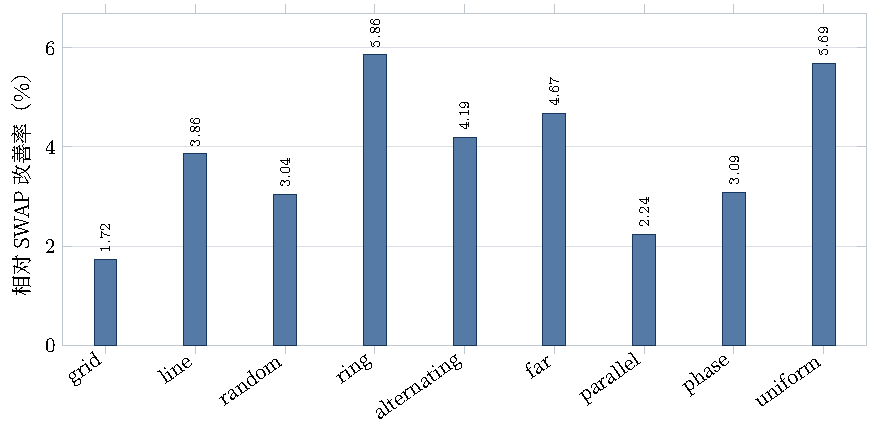
\includegraphics[width=0.96\textwidth]{figures/fig_v6_group_gain.pdf}
\caption{V6 拓扑与线路模式分组的相对 SWAP 改善}
\label{fig:group-gain}
\end{figure}

\subsection{规模与线路长度}

\begin{table}[H]
\centering
\small
\caption{V6 按量子比特数与长度因子分组}
\label{tab:size-length}
\begin{tabular}{llrrrrrr}
\toprule
分组 & 值 & 实例 & LightSABRE & 最终选择 & 减少 & 改善率 & 胜/平/负 \\
\midrule
\multirow{3}{*}{量子比特数}
 & 6  & 40 & 489  & 433  & 56 & 11.45\% & 21/19/0 \\
 & 8  & 40 & 1125 & 1087 & 38 & 3.38\%  & 16/24/0 \\
 & 10 & 40 & 1562 & 1531 & 31 & 1.98\%  & 13/27/0 \\
\midrule
\multirow{3}{*}{长度因子}
 & 3  & 40 & 392  & 378  & 14 & 3.57\% & 9/31/0 \\
 & 6  & 40 & 858  & 823  & 35 & 4.08\% & 18/22/0 \\
 & 12 & 40 & 1926 & 1850 & 76 & 3.95\% & 23/17/0 \\
\bottomrule
\end{tabular}
\end{table}

组合器在 6 比特实例上的相对改善达到 11.45\%，随后随规模增大而下降。当前一换位邻域在 $n$ 个逻辑比特上有 $\binom n2$ 个候选，虽仍可枚举，但每个布局只保留 4 个邻居；当 $n$ 增大时，这一固定预算覆盖的局部空间比例迅速下降。另一方面，三个长度因子的改善率均在 3.57\%--4.08\% 之间，显示结果并非只由最长线路贡献。

\subsection{正确性与执行等价}

\begin{table}[H]
\centering
\small
\caption{最终正确性与持久执行审计}
\label{tab:audit}
\begin{tabularx}{\textwidth}{p{0.42\textwidth}C{2.3cm}Y}
\toprule
审计项 & V6 结果 & 解释 \\
\midrule
语义等价 & 120/120 & Clifford 表示与期望物理线路完全相等。\\
拓扑合法 & 120/120 & 所有导出双比特门均位于硬件边。\\
指标一致 & 120/120 & 重算深度及 SWAP/CX 计数与选择记录一致。\\
持久执行主字段差异 & 0 & 选中后端、SWAP、深度与冻结质量结论不变。\\
辅助字段差异 & 1 & 未选中展开候选深度 29$\rightarrow$27；单例重跑确认 27。\\
未确认辅助差异 & 0 & 最终一致性审计通过。\\
\bottomrule
\end{tabularx}
\end{table}

辅助差异揭示了一个值得保留的复现细节：即使随机种子冻结，缓存预热和进程内执行顺序仍可能改变某些未选中候选的确定性破平轨迹。本文没有修改原始盲测主结果来追求“零差异”，而是将主字段与辅助字段分级，并用独立单例确认差异方向。这一处理避免以工程重跑覆盖预注册证据。

\subsection{独立公开环境复现}

% Public paper table reconstructed from the independently verified evidence.
\begin{table}[H]
\centering
\small
\caption{独立环境中的完整质量复现}
\label{tab:independent-reproduction}
\begin{tabular}{lrrrrrr}
\toprule
数据集 & 实例 & LightSABRE & SMPR & 减少 & 墙钟/s & 质量差异 \\
\midrule
V5 & 60 & 1691 & 1641 & 50 & 195.156 & 0 \\
V6 & 120 & 3176 & 3051 & 125 & 527.188 & 0 \\
\bottomrule
\end{tabular}
\end{table}


2026-07-25 在全新的 Windows 发布目录和隔离 Python 环境中，配置冻结依赖后
依次完成五例冒烟测试、完整 V5、完整 V6 和联合统计审计。V5 使用逐字段严格
策略，V6 使用只排除已隔离辅助深度字段的主质量策略；两者质量差异数均为 0。
公开候选包的本次完整运行分别用时 195.156\,s 和 527.188\,s；这些数值用于
证明独立环境可执行，不与另一台机器或另一版本解释器上的绝对时间直接比较。
联合审计重新得到实例级区间
$[-0.024346,-0.013634]$ 和因子单元区间
$[-0.024392,-0.013594]$，最终状态为 \texttt{PASSED: True}。

独立验证证据 ZIP 的 SHA-256 为
\texttt{6c7f38ae...c9af3a85d}。验证程序将清单中的原机器绝对路径映射到
本地证据根后，重新计算 18 个文件的哈希，18/18 一致；正式公开核心则重新
生成不含旧内部名称的逐实例表和描述性模块接口。证据复现包继续保存原始字段，
用于逐字节追踪；公开核心不把这些内部名称暴露为 API。

\subsection{持久分片运行时间}

\begin{table}[H]
\centering
\small
\caption{相同组合实现的执行方式比较}
\label{tab:runtime}
\begin{tabular}{llrrrr}
\toprule
数据集 & 原执行方式 & 原墙钟/s & 持久分片/s & 加速比 & 降幅 \\
\midrule
V5 & 每实例独立进程 & 212.569 & 78.975 & $2.692\times$ & 62.85\% \\
V6 & 顺序执行 & 583.840 & 200.207 & $2.916\times$ & 65.71\% \\
\bottomrule
\end{tabular}
\end{table}

V5 四分片完成时间为 69.00--78.97\,s，有实测代价支持的 LPT 取得较好平衡；有效并行度为 3.764。V6 无逐例时间参考，四分片完成时间为 139.60--200.16\,s，有效并行度为 3.382。两组结果表明，持久进程既减少了启动成本，也通过并行缩短墙钟。

然而，表~\ref{tab:runtime} 的基准不是“单独 LightSABRE”。SMPR 需要运行 20 个 LightSABRE、独立展开候选和若干跨布局候选，计算预算天然更高。故正确表述是“持久分片相对旧组合执行器加速 $2.7$--$2.9\times$”，而不是“SMPR 比 LightSABRE 快”。

\section{V7 前瞻性外部验证}

\subsection{研究问题与冻结边界}

V5/V6 证明了冻结合成分布上的质量改善，但没有覆盖公共程序、heavy-hex、
超过 10 个逻辑量子比特或同机质量--时间前沿。为此，公开核心带有独立的
V7 前瞻性规程。V7 不是继续调参的数据集；在观察任何路由结果前，线路清单、
源文件哈希、拓扑映射、SMPR 参数、确定性破平规则、重复次数、时间比例、
统计单位与失败报告规则必须共同存入只读冻结清单。若准备或运行失败，也必须
作为结果保留，不能通过替换线路或修改参数消除。

\begin{notebox}[title={V7 冻结与执行状态}]
V7 在观察路由结果前冻结 82 个输入、核心源码和协议文件，冻结清单 SHA-256 为
\texttt{90c4fb2b...2414901d}。三次同机重复、120 条配对观测、三个重复结果
哈希、三个环境记录及最终分析均已完成并通过。V7 数值只用于外部有效性和
质量--时间讨论，不改变 V6 的预注册主要推断，也不用于重新选择参数。
\end{notebox}

\subsection{公共线路与 heavy-hex 拓扑}

V7 从 QASMBench 的固定提交中选择 10 条公开 OpenQASM 2 线路
\citep{Li2022QASMBench}，覆盖可满足性、算术、机器学习、量子内存、
Bernstein--Vazirani、cat state 与 GHZ。所有源文件逐一记录 SHA-256，并随
上游许可证和说明文件归档。表~\ref{tab:v7-circuits} 给出预冻结清单。

\begin{table}[H]
\centering
\small
\caption{V7 冻结公共线路与目标 heavy-hex}
\label{tab:v7-circuits}
\begin{tabular}{lllrr}
\toprule
编号 & QASMBench 线路 & 类型 & 逻辑比特 & 物理比特 \\
\midrule
1  & \texttt{sat\_n11}        & 可满足性 & 11 & 19 \\
2  & \texttt{multiply\_n13}   & 算术 & 13 & 19 \\
3  & \texttt{bv\_n14}         & Bernstein--Vazirani & 14 & 19 \\
4  & \texttt{multiplier\_n15} & 算术 & 15 & 19 \\
5  & \texttt{dnn\_n16}        & 机器学习 & 16 & 19 \\
6  & \texttt{bigadder\_n18}   & 算术 & 18 & 19 \\
7  & \texttt{bv\_n19}         & Bernstein--Vazirani & 19 & 19 \\
8  & \texttt{qram\_n20}       & 量子内存 & 20 & 57 \\
9  & \texttt{cat\_state\_n22} & cat state & 22 & 57 \\
10 & \texttt{ghz\_state\_n23} & GHZ & 23 & 57 \\
\bottomrule
\end{tabular}
\end{table}

目标耦合图由 Qiskit \texttt{CouplingMap.from\_heavy\_hex} 生成
\citep{JavadiAbhari2024Qiskit,IBMHeavyHex}。11--19 逻辑比特映射到距离
$d=3$ 的 19 比特双向 heavy-hex，20--23 逻辑比特映射到距离 $d=5$ 的
57 比特图；物理规模满足
\begin{equation}
  N_{\mathrm p}=\frac{5d^2-2d-1}{2}.
\end{equation}
逻辑比特少于物理比特时允许使用空闲节点。该设计把规模外推与拓扑外推同时
纳入，但不混入设备误差率、校准变化或有向门代价，因而仍属于抽象连通性验证。

\subsection{线路规范化与正确性口径}

准备程序只删除最终测量和 barrier；发现中途测量、reset、经典条件或控制流
即拒绝。剩余线路在无耦合约束下以优化等级 0、固定种子 0 分解为
\texttt{u+cx}。路由只依赖门的量子比特占用与 DAG 顺序而不依赖一比特旋转
参数，因此程序进一步生成路由交互序列：全部 CX 和依赖顺序保持不变，每个一比特
操作替换为 $H$ 占位。源 QASM、规范化 QPY/QASM、路由交互序列数据与冻结配置
分别计算哈希。

V7 的正确性判据是映射单射、全部逻辑门恰执行一次、依赖顺序成立、最终映射
一致、所有物理 CX/SWAP 位于 heavy-hex 边，以及计数与选中候选一致。该审计
针对路由交互序列；它不能表述为对原始非 Clifford 程序的完整全线路等价证明。

\subsection{同机质量--时间前沿}

每条线路在同一物理机器、同一 Python/Qiskit 环境、同一线程限制下顺序运行
三次。每次先执行一次不计时的 LightSABRE 预热，再计时 SMPR 的候选生成与
确定性选择；文件导出和统计分析不计入核心时间。随后 LightSABRE 使用从 0
开始的确定性种子流连续运行，分别在 $0.25T$、$0.5T$、$T$ 与 $2T$ 的预算
处记录当前最优质量，其中 $T$ 是该次 SMPR 核心时间。每个预算至少包含
20 次 LightSABRE 试验，最多 10\,000 次。

每个观测记录 $(\mathrm{SWAP},\DepthW)$、墙钟、试验数、候选数、峰值 RSS、
CPU 与线程环境、路由审计和失败信息。主要比较以公共线路为组，将同一线路的
三次重复整体保留；每个时间比例报告总 SWAP、逐线路胜/平/负、重复方差与
10\,000 次 cluster bootstrap 区间。最小验收条件是 10 个源哈希一致、
120 个“线路$\times$重复$\times$预算”观测完整、全部线路大于 10 比特、
全部采用 heavy-hex、路由轨迹和拓扑审计全通过，以及 SMPR 相对其内部
20-seed LightSABRE 候选零 SWAP 退化。验收条件不要求 SMPR 在时间匹配基线
上获胜；负结果同样必须报告。

\subsection{完整性审计与质量--时间结果}

V7 实际获得 $10\times3\times4=120$ 条观测。冻结清单在三个重复环境中
完全一致，三个重复目录的结果清单均通过 SHA-256；路由轨迹、拓扑合法性和
SMPR 内部 20-seed LightSABRE 质量下界均为 120/120。上传证据包共含
29 个文件，其总清单以及分析目录、冻结目录和三个重复目录的嵌套清单全部
通过；在独立目录重跑分析器后，生成的 \texttt{summary.json} 与
\texttt{REPORT.md} 和原结果逐字节一致。

\begin{table}[H]
\centering
\small
\caption{V7 同机质量--时间前沿（三次重复合计）}
\label{tab:v7-frontier}
\begin{tabular}{rrrrrr}
\toprule
LS 预算 & SMPR SWAP & LS SWAP & 减少 & 相对减少 & 胜/平/负 \\
\midrule
$0.25T$ & 990 & 1113 & 123 & 11.05\% & 12/15/3 \\
$0.50T$ & 990 & 1086 &  96 &  8.84\% & 12/10/8 \\
$1.00T$ & 990 & 1068 &  78 &  7.30\% & 12/9/9 \\
$2.00T$ & 990 & 1044 &  54 &  5.17\% & 12/6/12 \\
\bottomrule
\end{tabular}
\end{table}

\begin{figure}[H]
\centering
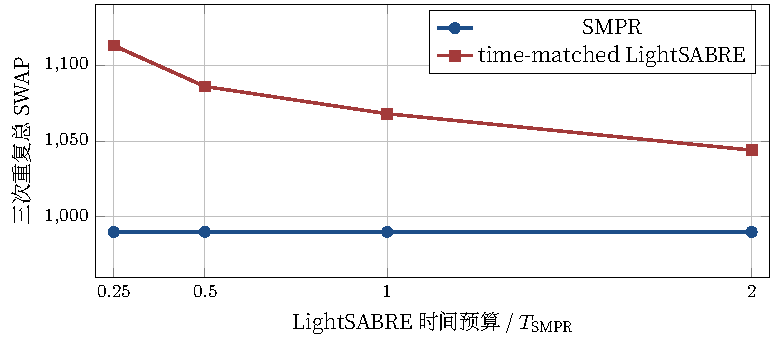
\includegraphics[width=0.80\textwidth]{figures/fig_v7_frontier.pdf}
\caption{V7 中 LightSABRE 随时间预算增加而改善，SMPR 的汇总优势相应收窄}
\label{fig:v7-frontier}
\end{figure}

差值按 $\mathrm{SMPR}-\mathrm{LightSABRE}$ 定义。四档预算的线路聚类
bootstrap 95\% 区间依次为
$[-0.359055,0.000724]$、$[-0.319770,0.005950]$、
$[-0.309690,0.015227]$ 和 $[-0.241537,0.023733]$。点估计均有利于
SMPR，且总量优势随 LightSABRE 预算增加而有规律地收窄；但所有区间都包含
零。因此，V7 证明协议执行和审计链完整，并提供跨公共线路、规模和 heavy-hex
拓扑的正向外部证据，却没有达到按线路聚类后 95\% 水平的显著性门槛。造成
区间较宽的主要原因是公共线路簇只有 10 个且线路类型差异较大，三次重复不能
替代更多独立线路。

\section{讨论}

\subsection{为什么独立展开较弱，组合仍然有效}

独立展开分支的完整 rollout 优化给定布局下的动作，但布局池本身仍可能与 LightSABRE 的双向、多试验布局质量存在差距。V6 中独立展开分支比 LightSABRE 多 210 个 SWAP，说明更深的路由决策不能自动补偿较弱布局。跨布局迁移把二者分解为两个可组合能力：LightSABRE 负责发现高质量布局，展开策略负责以不同方式重解释该布局及局部邻域。最终跨布局分支选中 51 例，证明布局迁移不是形式上的冗余分支。

这一结果也解释了本文为何把最终方法定义为 SMPR，而不以某个内部候选生成器命名：3.94\% 是整个候选组合、跨布局迁移与安全选择共同产生的结果，不能归因于独立展开分支。

\subsection{安全性与最优性的区别}

命题 1 只保证相对候选集内 LightSABRE 的不退化，不保证全局最优，也不保证相对其他未包含路由器的优势。该安全性还依赖两个工程前提：LightSABRE 候选必须真实保留，且所有候选必须使用一致的 SWAP 与深度口径。三重审计正是为了将形式选择规则落实到导出线路。

完整策略展开也不是精确动态规划。它只在启发式前 $k$ 个候选上计算基线策略的完整余值，并在每一步重新规划；结果仍受候选覆盖、基线策略和缓存指纹影响。其优势在于用可控预算减少启发式后悔，而非穷举所有交换序列。

\subsection{内部有效性威胁}

\begin{itemize}[itemsep=0.30em]
  \item \textbf{缓存与执行顺序：}V6 的 1 个辅助深度差异表明，未选中候选可受缓存预热轨迹影响。主字段已通过独立审计，但未来实现应将所有破平所需状态显式纳入指纹。
  \item \textbf{统计单位：}120 个 V6 实例来自 60 个因子单元的两个随机实现，不能视为无限独立的真实应用分布。bootstrap 反映该构造分布上的配对稳定性。
  \item \textbf{选择偏差：}V5 参与了冻结等价和工程检查，因此本文不把 V5 作为独立确认性证据。主要推断只来自冻结后生成的 V6。
  \item \textbf{环境记录：}公开包已固定 Python 兼容区间、Qiskit 2.4.2 和 OpenQASM 3 导入器 0.6.0，并在隔离 Windows 环境完成独立全量复现；但原冻结计时缺少 CPU 型号，绝对时间仍不可跨平台比较。
\end{itemize}

\subsection{外部有效性与后续工作}

V7 将已有结果从 6--10 比特合成线路扩展到 10 条 11--23 比特 QASMBench
公共线路以及 19/57 比特 heavy-hex，并首次在同一机器上给出 SMPR 与
LightSABRE 的匹配预算前沿。四档预算的总 SWAP 均有利于 SMPR，说明 V6
观察到的组合收益没有在拓扑和规模外推后立即消失；与此同时，cluster 区间
跨零表明外部样本仍不足以支持普遍优势。带方向和误差率的真实设备拓扑、
动态线路、更多公共套件以及原始非 Clifford 线路的端到端等价仍需后续验证。

固定保留 4 个一换位邻居在 6 比特时覆盖比例较高，在 10 比特时相对不足。可研究按 $\binom n2$、代理分数间隔或在线收益自适应邻域预算。V6 无实测时间参考导致 LPT 尾部不平衡，未来可采用持久工作池和动态任务窃取，同时记录每个候选后端的细粒度时间，以建立质量--时间 Pareto 前沿。

\section{可复现性与证据治理}

算法冻结、盲测和执行优化按以下时间顺序分离：

\begin{enumerate}[label=\textbf{步骤 \arabic*:},leftmargin=5em,itemsep=0.35em]
  \item 在只使用开发数据的条件下固定组合参数：LightSABRE $20\times1$、全部并列最优布局、每布局 4 个邻居、代理衰减 0.95。
  \item 生成 V6 冻结清单，以该清单哈希派生随机种子，并在结果不可见时锁定主要统计规则。
  \item 生成并运行 120 例盲测；随后按预注册规则完成实例级 bootstrap，形成主要推断。
  \item 仅改变执行方式而不改变路由逻辑，并将最终质量字段与未选中候选的辅助字段分级审计。
  \item 汇总 V5/V6 质量、统计推断、运行时间与 SHA-256，形成不可变证据包。
  \item 增补因子单元 bootstrap、留一层级与逐实例复算，作为明确标注的事后稳健性检查。
  \item 在独立 Windows 环境重跑 V5/V6 和联合审计，验证证据包内 18 个文件哈希，并从完整研发过程构建正式公开核心。
  \item 在读取任何 V7 路由结果前冻结 82 个输入、协议和核心文件；随后完成三次同机重复、120 条匹配预算观测、嵌套哈希审计和独立分析复算。
\end{enumerate}

\begin{table}[H]
\centering
\small
\caption{论文、程序与证据交付物}
\label{tab:artifacts}
\begin{tabularx}{\textwidth}{p{0.34\textwidth}Y}
\toprule
文件 & 用途 \\
\midrule
\texttt{quality\_summary.csv} & V5/V6 总质量、胜平负、审计和后端选择分布。\\
\texttt{runtime\_summary.csv} & 旧执行方式与持久分片的墙钟、加速比和重启减少数。\\
\texttt{v6\_group\_summary.csv} & 拓扑、线路模式、规模与长度因子的分组结果。\\
\texttt{manifest.json} & 输入哈希、输出哈希、最终数值和通过状态。\\
\texttt{SHA256SUMS.txt} & 最终证据文件完整性校验。\\
\texttt{FINAL\_EVIDENCE\_REPORT.md} & 结论层级与论文表述边界。\\
\texttt{reliability\_audit/} & 逐实例结构复算、cluster bootstrap 与留一层级稳定性。\\
\texttt{verified\_evidence/} & 独立环境复现的原始结果、环境和联合审计。\\
\texttt{v7\_verified\_evidence/} & V7 冻结清单、三次配对前沿、环境记录、分析报告与嵌套哈希。\\
\texttt{SMPR\_quantum\_router\_public/} & 无旧内部名称的公开核心、V7 规程、测试与统一命令行。\\
\texttt{SMPR\_history\_archive/} & 完整研发过程、原始字段、数据、运行记录及逐文件哈希。\\
\texttt{SOURCE\_MANIFEST.json} & 公开核心文件大小和 SHA-256。\\
\bottomrule
\end{tabularx}
\end{table}

论文统计只使用第一次冻结运行的 V6 质量结果；持久执行和独立环境重跑仅验证
执行等价、可用性与新墙钟。任何后续算法改动都必须提升版本号并使用新的未见
数据，不能继续把 V6 解释为盲测。V7 已按前瞻协议冻结并完成，其结果只能按
表~\ref{tab:v7-frontier} 和对应 cluster 区间陈述；若继续调整算法，则必须
另建未见数据集，不能用当前 V7 反复调参。

\section{结论}

本文提出并验证了 SMPR：一个以 LightSABRE 为显式质量下界、以完整策略展开和跨布局重路由为互补搜索的安全多布局组合路由器。它把“更深搜索是否总能击败强基线”转化为更稳健的问题：如何在保留强基线的同时，只接受经真实完整路由证明更好的候选。冻结后的 V6 预注册盲测显示，总 SWAP 从 3176 降至 3051，改善 3.94\%，逐实例为 50/70/0；归一化配对差值的 bootstrap 95\% 区间完全低于零，且 120 个实例全部通过语义、拓扑和指标审计。

V7 又在 10 条公共线路、11--23 逻辑比特和 heavy-hex 上给出同机质量--时间
前沿：SMPR 在四档预算下减少 5.17\%--11.05\% 的总 SWAP，全部完整性与
路由审计通过；不过线路聚类区间均跨零，因此该部分是正向外部证据而非新的
显著性结论。结果同样给出清晰的否定结论：独立展开分支弱于 LightSABRE，
最终收益主要来自安全组合和布局迁移；持久分片改善的是组合实现的工程效率，
不等同于证明组合方法在任意线路上快于 LightSABRE。

\section*{致谢}

本节待作者补充。建议说明计算资源、代码贡献、数据审计与资助信息；若无相关内容，可在投稿前删除。

\section*{数据与代码可用性}

交付物分为三部分：正式中文论文及实验报告；不含旧内部名称的 SMPR 公开核心；
完整研发过程复现包。公开核心提供冻结配置、统一命令行、自检、单元测试、
断点恢复、公开字段导出和 V7 预注册脚本；研发过程字段和编号脚本只在独立复现包中
保留，用于证据兼容，不作为正式算法命名。完整复现固定 Qiskit 2.4.2 和
qiskit-qasm3-import 0.6.0，并应同时记录 Python、操作系统、CPU 型号、线程
环境与所有命令行参数。V7 公共线路来自固定 QASMBench 提交并带有上游许可证；
V7 证据包 SHA-256 为
\texttt{a8e21b91...8b9a9a75}，包含冻结清单、三个重复结果、环境记录、
分析报告与逐文件哈希。

\begingroup
\sloppy
\raggedright
\bibliographystyle{unsrtnat}
\bibliography{references}
\endgroup

\appendix

\section{术语与结果口径速查}

\begin{longtable}{p{0.27\textwidth}p{0.66\textwidth}}
\caption{本文术语的严格含义}\label{tab:terminology}\\
\toprule
术语 & 含义 \\
\midrule
\endfirsthead
\toprule
术语 & 含义 \\
\midrule
\endhead
LightSABRE & 每例 20 个 Qiskit SABRE 自动布局/路由种子中按 $(S,\DepthW)$ 选出的最佳候选。\\
独立展开分支 & 使用自身冻结自适应布局策略和完整基线策略展开的候选；不使用 LightSABRE 布局。\\
双分支选择 & 只在 LightSABRE 最优候选与独立展开候选之间按质量取优。\\
跨布局分支 & 从 LightSABRE 并列最优初始布局及其代理前 4 一换位邻居出发，重新运行完整展开路由。\\
SMPR 最终选择 & 在 LightSABRE、独立展开和跨布局候选上按式~\eqref{eq:deterministic-key} 取优；冻结 V5/V6 使用式~\eqref{eq:frozen-key}。\\
SWAP 胜/平/负 & 只比较每例最终选择与 LightSABRE 的 SWAP。\\
质量胜/平/负 & 比较每例 $(S,\DepthW)$ 字典序。\\
运行时间加速 & 旧组合执行方式相对四个持久分片的墙钟比；不是相对单独 LightSABRE。\\
\bottomrule
\end{longtable}

\section{论文主张检查表}

\begingroup
\setlength{\tabcolsep}{4pt}
\renewcommand{\arraystretch}{0.90}
\begin{table}[H]
\centering
\footnotesize
\caption{可使用与不可使用的论文表述}
\label{tab:claim-checklist}
\begin{tabularx}{\textwidth}{C{1.2cm}Y}
\toprule
状态 & 表述 \\
\midrule
\textcolor{GainGreen}{可使用} &
“在冻结后的 120 例 V6 预注册盲测上，安全组合相对 20-seed LightSABRE 减少 3.94\% 总 SWAP，逐实例无 SWAP 退化。”\\
\textcolor{GainGreen}{可使用} &
“平均归一化配对差值的 10\,000 次 bootstrap 95\% 区间为 $[-0.024346,-0.013634]$。”\\
\textcolor{GainGreen}{可使用} &
“四个持久分片相对旧组合执行方式在 V6 上取得 $2.916\times$ 墙钟加速。”\\
\textcolor{WarnRed}{不可使用} &
“独立展开分支的路由质量优于 LightSABRE。”该分支在 V6 多 210 个 SWAP。\\
\textcolor{WarnRed}{不可使用} &
“本文组合路由器比 LightSABRE 更快。”现有运行时间基准未进行该比较。\\
\textcolor{WarnRed}{不可使用} &
“在任意量子线路和硬件拓扑上保证改善。”现有结论限于冻结候选集和 V6 构造分布。\\
\bottomrule
\end{tabularx}
\end{table}
\endgroup

\end{document}
